\documentclass[tikz, border=1mm]{standalone}

%Packages
\usepackage{xcolor} %Advanced colors
\usetikzlibrary{calc} %para calculos da grade
\usetikzlibrary{angles,quotes} %Para calcular seno e cosseno
%\usepackage{tikz-3dplot} %Enable 3d plot
\usepackage{pgfmath} % Advanced calculus
\usetikzlibrary{math}

%Pallet colors
\definecolor{spinUP}{HTML}{181818}
\colorlet{spinDOWN}{white}
%\definecolor{spinDOWN}{HTML}{F5F5F5}
\definecolor{cluster}{HTML}{F2D57E}
\definecolor{j1}{HTML}{D72C01}
\definecolor{j2}{HTML}{F3ECD1}
\definecolor{j3}{HTML}{A72504}
\definecolor{j4}{HTML}{00746E}

%Parameters
%size lattice
\newcommand{\Lx}{3} %Size lattice
\newcommand{\Ly}{3}
\newcommand{\LL}{3} %if Lx = Ly
\newcommand{\lw}{0.01cm} %line width
\pgfmathsetmacro\rebarba{0.005} %lw/2



%Faça este valor sempre=\nSitios-1 
\newcommand{\sizeCircle}{12pt}
\newcommand{\sizeFont}{\LARGE}
\newcommand{\translate}{-2}
\newcommand{\translateY}{3.2}
\newcommand{\translateLegend}{0.}
\newcommand{\translateCLUSTERS}{3}
\newcommand{\translateFigb}{-2.96,-1.7}
\newcommand{\translateFigc}{-0.66,-0.5}
\newcommand{\factorSizeLattice}{0.6}
% Calcula a divisão de \nSitios por 2, e trunca num inteiro
\pgfmathtruncatemacro{\nClusters}{\Lx/2}

\begin{document}
	%%%%%%%%%%%%%%%%%
%%  Styles							  %%
%%  M. Roos, 25/03/2025	 %%
%%%%%%%%%%%%%%%%%

% Circles with shadow and glow
\begin{tikzpicture}
	\draw[step=1cm, line width=1] (0,0) grid (\LL, \LL);
	\foreach \j in {0,1,...,\LL}{
		\foreach \i in {0,1,...,\LL}{
			\fill[ball color=j4, shading angle=\povGlow] (\i,\j) circle(\sizeCircle) ; 
			}
		}
	\node at (1.5,3.3) {\tiny Circles with shadow and glow};
\end{tikzpicture}

% Help lines style
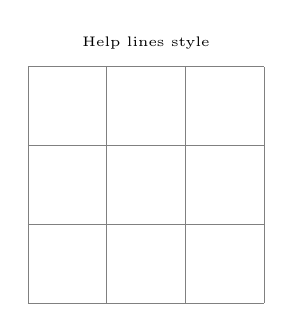
\begin{tikzpicture}
	\draw[help lines] (0,0) grid (3,3);
	\node at (1.5,3.3) {\tiny Help lines style};
\end{tikzpicture}

% Help lines style: add style
\begin{tikzpicture}
	\tikzstyle{help lines}+=[dashed]
	\draw[help lines] (0,0) grid (3,3);
	\node at (1.5,3.3) {\tiny Add style};
\end{tikzpicture}

% Round extreme
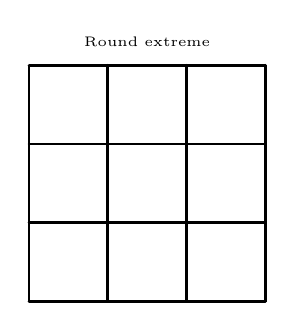
\begin{tikzpicture}
	\draw[line width=1, line cap=round] (0,0) grid (3,3);
	\node at (1.5,3.3) {\tiny Round extreme};
\end{tikzpicture}

% MyStyle
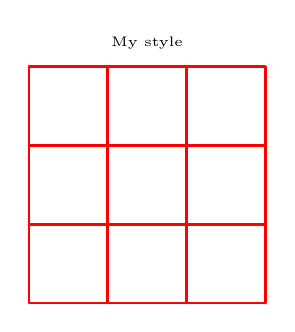
\begin{tikzpicture}
	[myStyle/.style={draw=red, line width=1, line cap=round}]
	\draw[myStyle] (0,0) grid (3,3);
	\node at (1.5,3.3) {\tiny My style};
\end{tikzpicture}

% Create my personal style with condition
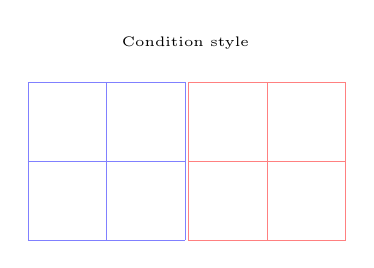
\begin{tikzpicture}
	[myStyle/.style ={help lines,color=#1!50},
	myStyle/.default=blue]
	\draw[myStyle] (0,0) grid (2,2);
	\draw[myStyle=red, xshift=1] (2,0) grid (4,2);
	\node at (2,2.5) {\tiny Condition style};
\end{tikzpicture}

% My style for grid and spins with node
\begin{tikzpicture}
	\draw[myGrid] (0,0) grid (\LL, \LL);
	\foreach \j in {0,1,...,\LL}{
		\foreach \i in {0,1,...,\LL}{
			\node[mySpin] at (\i,\j) {} ; 
		}
	}
	\node at (1.5,3.3) {\tiny My lattice};
\end{tikzpicture}


\end{document}